\iffalse
\documentclass[journal,12pt,twocolumn]{IEEEtran}
%
\usepackage{setspace}
\usepackage{gensymb}
%\doublespacing
\singlespacing

%\usepackage{graphicx}
%\usepackage{amssymb}
%\usepackage{relsize}
\usepackage[cmex10]{amsmath}
%\usepackage{amsthm}
%\interdisplaylinepenalty=2500
%\savesymbol{iint}
%\usepackage{txfonts}
%\restoresymbol{TXF}{iint}
%\usepackage{wasysym}
\usepackage{amsthm}
%\usepackage{iithtlc}
\usepackage{mathrsfs}
\usepackage{txfonts}
\usepackage{stfloats}
\usepackage{bm}
\usepackage{cite}
\usepackage{cases}
\usepackage{subfig}
%\usepackage{xtab}
\usepackage{longtable}
\usepackage{multirow}
%\usepackage{algorithm}
%\usepackage{algpseudocode}
\usepackage{enumitem}
\usepackage{mathtools}
\usepackage{steinmetz}
\usepackage{tikz}
\usepackage{circuitikz}
\usepackage{verbatim}
\usepackage{tfrupee}
\usepackage[breaklinks=true]{hyperref}
%\usepackage{stmaryrd}
\usepackage{tkz-euclide} % loads  TikZ and tkz-base
%\usetkzobj{all}
\usetikzlibrary{calc,math}
\usepackage{listings}
    \usepackage{color}                                            %%
    \usepackage{array}                                            %%
    \usepackage{longtable}                                        %%
    \usepackage{calc}                                             %%
    \usepackage{multirow}                                         %%
    \usepackage{hhline}                                           %%
    \usepackage{ifthen}                                           %%
  %optionally (for landscape tables embedded in another document): %%
    \usepackage{lscape}     
\usepackage{multicol}
\usepackage{chngcntr}
%\usepackage{enumerate}

%\usepackage{wasysym}
%\newcounter{MYtempeqncnt}
\DeclareMathOperator*{\Res}{Res}
%\renewcommand{\baselinestretch}{2}
\renewcommand\thesection{\arabic{section}}
\renewcommand\thesubsection{\thesection.\arabic{subsection}}
\renewcommand\thesubsubsection{\thesubsection.\arabic{subsubsection}}

\renewcommand\thesectiondis{\arabic{section}}
\renewcommand\thesubsectiondis{\thesectiondis.\arabic{subsection}}
\renewcommand\thesubsubsectiondis{\thesubsectiondis.\arabic{subsubsection}}

% correct bad hyphenation here
\hyphenation{op-tical net-works semi-conduc-tor}
\def\inputGnumericTable{}                                 %%

\lstset{
%language=C,
frame=single, 
breaklines=true,
columns=fullflexible
}
%\lstset{
%language=tex,
%frame=single, 
%breaklines=true
%}

\begin{document}
%


\newtheorem{theorem}{Theorem}[section]
\newtheorem{problem}{Problem}
\newtheorem{proposition}{Proposition}[section]
\newtheorem{lemma}{Lemma}[section]
\newtheorem{corollary}[theorem]{Corollary}
\newtheorem{example}{Example}[section]
\newtheorem{definition}[problem]{Definition}
%\newtheorem{thm}{Theorem}[section] 
%\newtheorem{defn}[thm]{Definition}
%\newtheorem{algorithm}{Algorithm}[section]
%\newtheorem{cor}{Corollary}
\newcommand{\BEQA}{\begin{eqnarray}}
\newcommand{\EEQA}{\end{eqnarray}}
\newcommand{\define}{\stackrel{\triangle}{=}}

\bibliographystyle{IEEEtran}
%\bibliographystyle{ieeetr}


\providecommand{\mbf}{\mathbf}
\providecommand{\pr}[1]{\ensuremath{\Pr\left(#1\right)}}
\providecommand{\qfunc}[1]{\ensuremath{Q\left(#1\right)}}
\providecommand{\sbrak}[1]{\ensuremath{{}\left[#1\right]}}
\providecommand{\lsbrak}[1]{\ensuremath{{}\left[#1\right.}}
\providecommand{\rsbrak}[1]{\ensuremath{{}\left.#1\right]}}
\providecommand{\brak}[1]{\ensuremath{\left(#1\right)}}
\providecommand{\lbrak}[1]{\ensuremath{\left(#1\right.}}
\providecommand{\rbrak}[1]{\ensuremath{\left.#1\right)}}
\providecommand{\cbrak}[1]{\ensuremath{\left\{#1\right\}}}
\providecommand{\lcbrak}[1]{\ensuremath{\left\{#1\right.}}
\providecommand{\rcbrak}[1]{\ensuremath{\left.#1\right\}}}
\theoremstyle{remark}
\newtheorem{rem}{Remark}
\newcommand{\sgn}{\mathop{\mathrm{sgn}}}
\providecommand{\abs}[1]{\left\vert#1\right\vert}
\providecommand{\res}[1]{\Res\displaylimits_{#1}} 
\providecommand{\norm}[1]{\left\lVert#1\right\rVert}
%\providecommand{\norm}[1]{\lVert#1\rVert}
\providecommand{\mtx}[1]{\mathbf{#1}}
\providecommand{\mean}[1]{E\left[ #1 \right]}
\providecommand{\fourier}{\overset{\mathcal{F}}{ \rightleftharpoons}}
%\providecommand{\hilbert}{\overset{\mathcal{H}}{ \rightleftharpoons}}
\providecommand{\system}{\overset{\mathcal{H}}{ \longleftrightarrow}}
	%\newcommand{\solution}[2]{\textbf{Solution:}{#1}}
\newcommand{\solution}{\noindent \textbf{Solution: }}
\newcommand{\cosec}{\,\text{cosec}\,}
\providecommand{\dec}[2]{\ensuremath{\overset{#1}{\underset{#2}{\gtrless}}}}
\newcommand{\myvec}[1]{\ensuremath{\begin{pmatrix}#1\end{pmatrix}}}
\newcommand{\mydet}[1]{\ensuremath{\begin{vmatrix}#1\end{vmatrix}}}
%\numberwithin{equation}{section}
\numberwithin{equation}{subsection}
%\numberwithin{problem}{section}
%\numberwithin{definition}{section}
\makeatletter
\@addtoreset{figure}{problem}
\makeatother

\let\StandardTheFigure\thefigure
\let\vec\mathbf
%\renewcommand{\thefigure}{\theproblem.\arabic{figure}}
\renewcommand{\thefigure}{\theproblem}
%\setlist[enumerate,1]{before=\renewcommand\theequation{\theenumi.\arabic{equation}}
%\counterwithin{equation}{enumi}


%\renewcommand{\theequation}{\arabic{subsection}.\arabic{equation}}

\def\putbox#1#2#3{\makebox[0in][l]{\makebox[#1][l]{}\raisebox{\baselineskip}[0in][0in]{\raisebox{#2}[0in][0in]{#3}}}}
     \def\rightbox#1{\makebox[0in][r]{#1}}
     \def\centbox#1{\makebox[0in]{#1}}
     \def\topbox#1{\raisebox{-\baselineskip}[0in][0in]{#1}}
     \def\midbox#1{\raisebox{-0.5\baselineskip}[0in][0in]{#1}}

\vspace{3cm}


\title{Question: 9.10.4.5}
\author{Nikam Pratik Balasaheb (EE21BTECH11037)}





% make the title area
\maketitle

\newpage

%\tableofcontents

\bigskip

\renewcommand{\thefigure}{\theenumi}
\renewcommand{\thetable}{\theenumi}
%\renewcommand{\theequation}{\theenumi}

\section{Problem}
Three girls Reshma, Salma and Mandip are playing a game by standing on a circle of radius 5m drawn in a park. Reshma throws a ball to Salma, Salma to Mandip, Mandip to Reshma. If the distance between Reshma and Salma and
between Salma and Mandip is 6m each, what is the distance between Reshma and Mandip?

\section{Solution}
\fi
Consider Reshma, Salma and Mandip be standing at $\vec{A}$, $\vec{B}$ and $\vec{C}$ respectively, and the center the of the circle $\vec{O}$.
The input parameters are listed in Table 
\ref{tab:chapters/9/10/4/5/}.
Let 
\begin{align}
	\vec{B} = \myvec{0\\0},\,
	\vec{O} = \myvec{5\\0}
\end{align}
Therefore, the equation of the cicle is given by 
\begin{align}
	\norm{\vec{x}-\vec{O}}^2 &= 25\\
\implies 	\norm{\vec{x}}^2 - 2 \vec{O}^{\top}\vec{x} + \norm{\vec{O}}^2 - 25 &= 0\\
\implies	\norm{\vec{x}}^2 - 2 \myvec{5 & 0}\vec{x} &= 0
	\label{eq:chapters/9/10/4/5/1}
\end{align}
Also, $\vec{A}$ and $\vec{C}$ are equidistant (6m) from $\vec{B}$, we can say that they lie on the circle having $\vec{B}$ as center and radius 6m. Equation of this circle is given by
\begin{align}
	\norm{\vec{x}}^2 - 2\vec{B}^{\top} \vec{x} + \norm{\vec{B}}^2 - 36 &= 0\\
	\norm{\vec{x}}^2 &= 36\\
	i.e., \vec{u} = \myvec{0\\0}\;, \; f = -36
	\label{eq:chapters/9/10/4/5/2}
\end{align}
From \eqref{eq:chapters/9/10/4/5/1} and \eqref{eq:chapters/9/10/4/5/2}, the line passing through $\vec{A}$ and $\vec{C}$  is
\begin{align}
	\myvec{5&0} \vec{x} &= 18\\
\implies 	\vec{x} &= \myvec{\frac{18}{5}\\[1pt] 0} + \mu \myvec{0\\1}\\
	i.e., \; \vec{h} = \myvec{\frac{18}{5}\\[1pt] 0} \; , \; \vec{m} = \myvec{0\\1}
\end{align}
For the circle,$\vec{V} = \vec{I}$
\begin{multline}
	\mu_i = \frac{1}{\vec{m}^{\top}\vec{V}\vec{m}} \brak{-m^{\top}\brak{\vec{V}\vec{h}+\vec{u}} \pm \sqrt{\brak{\vec{m}^{\top}\brak{\vec{V}\vec{h}+\vec{u}}}^2 - \text{g}\brak{\vec{h}}\brak{\vec{m}^{\top}\vec{V}\vec{m}}}}
\end{multline}
where,
\begin{align}
	\text{g}\brak{\vec{h}} = \vec{h}^{\top}\vec{V}\vec{h} + 2\vec{u}^{\top}\vec{h} +f
\end{align}
yielding
\begin{align}
	\mu_i = \pm \frac{24}{5}
\end{align}
Therefore,
\begin{align}
	\vec{A} = \myvec{\frac{18}{5}\\[1pt] \frac{24}{5}},\,
	\vec{C} = \myvec{\frac{18}{5}\\[1pt] -\frac{24}{5}}
\end{align}
and the 
distance between Reshma and Mandip is
\begin{align}
	\norm{\vec{A} - \vec{C}} = \norm{\myvec{0\\[1pt] \frac{48}{5}}}
	= \frac{48}{5}
\end{align}
\begin{table}[h!]
\begin{center}
	%%%%%%%%%%%%%%%%%%%%%%%%%%%%%%%%%%%%%%%%%%%%%%%%%%%%%%%%%%%%%%%%%%%%%%
%%                                                                  %%
%%  This is a LaTeX2e table fragment exported from Gnumeric.        %%
%%                                                                  %%
%%%%%%%%%%%%%%%%%%%%%%%%%%%%%%%%%%%%%%%%%%%%%%%%%%%%%%%%%%%%%%%%%%%%%%

\begin{tabular}[]{|c|c|c|}
\hline
$\vec{O}$	& $\myvec{5\\0}$ &Center of the given circle \\ \hline
$\vec{B}$	& $\myvec{0\\0}$ &Point where Salma is standing\\ \hline
$r$		& 5 & radius of given circle \\ \hline
$d$ 		& 6 & distance AB and BC\\ \hline
\end{tabular}

\end{center}
\caption{}
\label{tab:chapters/9/10/4/5/}
\end{table}
See Fig. 
    \ref{fig:chapters/9/10/4/5/}.
\begin{figure}[h!]
  \centering
    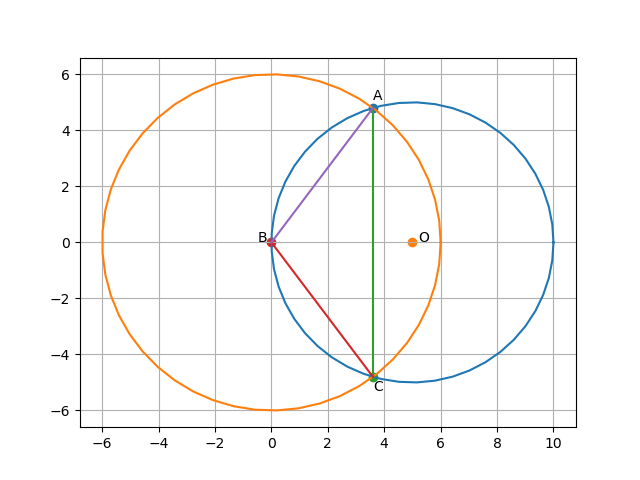
\includegraphics[width=\columnwidth]{chapters/9/10/4/5/figs/Figure_1.png}
    \caption{}
    \label{fig:chapters/9/10/4/5/}
\end{figure}




